\documentclass[a4paper,twocolumn,5p]{elsarticle}

\usepackage{hyperref}
%\usepackage{lineno}
%\modulolinenumbers[5]

\usepackage{booktabs}
\usepackage{graphicx}
\usepackage{xspace}
\usepackage{booktabs}
\usepackage[draft]{fixme}

\journal{Environment International}

%% `Elsevier LaTeX' style
\bibliographystyle{elsarticle-num}
%%%%%%%%%%%%%%%%%%%%%%%

\begin{document}

% Macro para escribir NO$_2$
\newcommand{\no}{NO\textsubscript{2}\xspace}

\begin{frontmatter}

\title{A comparison of probabilistic forecasting methods for extreme \no pollution episodes}

\author{Sebasti\'an P\'erez}
\address{(afiliaci\'on y direcci\'on)}

\author{Jos\'e L. Aznarte\fnref{myfootnote}}
\address{Artificial Intelligence Department\\Universidad Nacional de
  Educaci\'on a Distancia --- UNED\\c/ Juan del Rosal, 16, Madrid, Spain}
\ead{jlaznarte@dia.uned.es}

\fntext[myfootnote]{This work has been partially funded by Ministerio
  de Econom\'ia y Competitividad, Gobierno de Espa\~na, through a
  \emph{Ram\'on y Cajal} grant % awarded to Dr Aznarte
  (reference: RYC-2012-11984).}


\begin{abstract}

\end{abstract}

\begin{keyword}
probabilistic forecasting \sep air quality \sep quantile regression
\sep nitrogen dioxide \sep Madrid
\end{keyword}

\end{frontmatter}

%\linenumbers

\section{Introduction}
\label{sec:intro}



\section{Probabilistic forecasting with quantile regression}
\label{sec:probForec}

As mentioned above, the prediction from most regression models is a
point estimate of the conditional mean of a dependent variable, or
response, given a set of independent variables or predictors. However,
the conditional mean measures only the center of the conditional
distribution of the response, and if we need a more complete summary
of this distribution, for example in order to estimate the associated
uncertainty, quantiles are in order. The 0.5 quantile (i.e., the
median) can serve as a measure of the center, and the 0.9 quantile
marks the value of the response below which reside the 90\% of the
predicted points. Recent advances in computing have inducted the
development of regression models for predicting given quantiles of the
conditional distribution. The technique is called quantile regression
(QR) and was first proposed by Koenker in 1978
\cite{koenker_regression_1978} based on the intuitions of the
astronomer and polymath Rudjer Boscovich in the 18th
century. Elaborating from the same concept of estimating conditional
quantiles from different perspectives, several statistical and CI
models that implement this technique have been developed: from the
original linear proposal to multiple or additive regression, neural
networks, support vector machines, random forests etc.

Quantile regression has gained an increasing attention from very
different scientific disciplines \cite{yu_quantile_2003}, including
financial and economic applications \cite{fitzenberger_economic_2002},
medical applications \cite{soyiri_forecasting_2012}, wind power
forecasting \cite{zhang_review_2014}, electric load forecasting
\cite{7423794,gibbons_quantile_2014}, environmental modelling
\cite{cade_gentle_2003} and meteorological modelling
\cite{bjornar_bremnes_probabilistic_2004} (these references are just
examples and the list is not exhaustive). To our knowledge, despite
its success in other areas, quantile regression has not been applied
in the framework of air quality% , with the exception of
% \cite{martinez-silva_forecasting_2016}
.

As an illustration of the concept (for a detailed discussion of
quantile regression, refer to \cite{koenker_quantile_2005}), given a
set of vectors $(x_i, y_i)$, in point forecasting we are usually
interested in what prediction $\hat y(x) = \alpha_0 + \alpha_1 x$
minimizes the mean squared error,
\begin{equation}
  \label{eq:1}
  E = \frac{1}{n} \sum^n_i \epsilon_i =
  \frac{1}{n} \sum^n_i [ y_i - (\alpha_0 + \alpha_1 x) ]^2.
\end{equation}
This prediction is the conditional sample mean of $y$ given $x$% , that
% is, $\hat y(x) = \hat\alpha_0 + \hat\alpha_1 x$
, or the location of the conditional distribution. But we could be
interested in estimating the conditional median (i.e., the 0.5
quantile) instead of the mean, in which case we should find the
prediction $\hat y(x)$ which minimizes the mean absolute error,
\begin{equation}
  \label{eq:2}
  E = \frac{1}{n} \sum^n_i \epsilon_i =
  \frac{1}{n} \sum^n_i | y_i - (\alpha_0 + \alpha_1 x) |.
\end{equation}
The fact is that, apart from the 0.5 quantile, it is possible to
estimate any other given quantile $\tau$. In that case, instead of
(\ref{eq:2}), we could minimize
\begin{equation}
  \label{eq:3}
E= \frac{1}{n} \sum^n_i f( y_i - (\alpha_0 + \alpha_1 x))
\end{equation}
where
\begin{equation}
  \label{eq:4}
  f(y-q) = \left\{ 
\begin{array}{l l}
\tau (y-q) & \quad \mbox{if $y \ge q$}\\
(1-\tau) (q-y) & \quad \mbox{if $y < q$}\\
\end{array} \right.,
\end{equation}
with $\tau \in (0,1)$. Equation (\ref{eq:3}) represents the
median when $\tau=0.5$ and the $\tau$-th quantile in any other case.

Thus, as we can estimate an arbitrary quantile and forecast its
values, we can also estimate the full conditional distribution, which
will entail us to the results presented in Section \ref{sec:results}.

Among the array of methods that allow to estimate and forecast
data-driven conditional quantiles, in this study we have chosen
quantile regression forests for its ease of use (few parameters have
to be chosen) and for its availability in the free software
mathematical environment \texttt{R} \cite{r-language}.
For a detailed discussion on quantile regression forests, see
\cite{meinshausen_quantile_2006}.

\section{Data description and experimental design}

\subsection{k-Neighbors}


The probabilistic k-Neighbors is based on the competition entry from [K-nearest neighbors for GEFCom2014 probabilistic wind power forecasting]. We are using a k-neighbor algorithm, where instead of aggregating the targets for those k-neighbors (by taking the mean or the median), we are calculating the quantiles of those targets.

We then use the CRPS of our distribution estimation to get the best number of k-neighbor. As you can see in the chart, we chose 50 as the optimal number of neighbor.

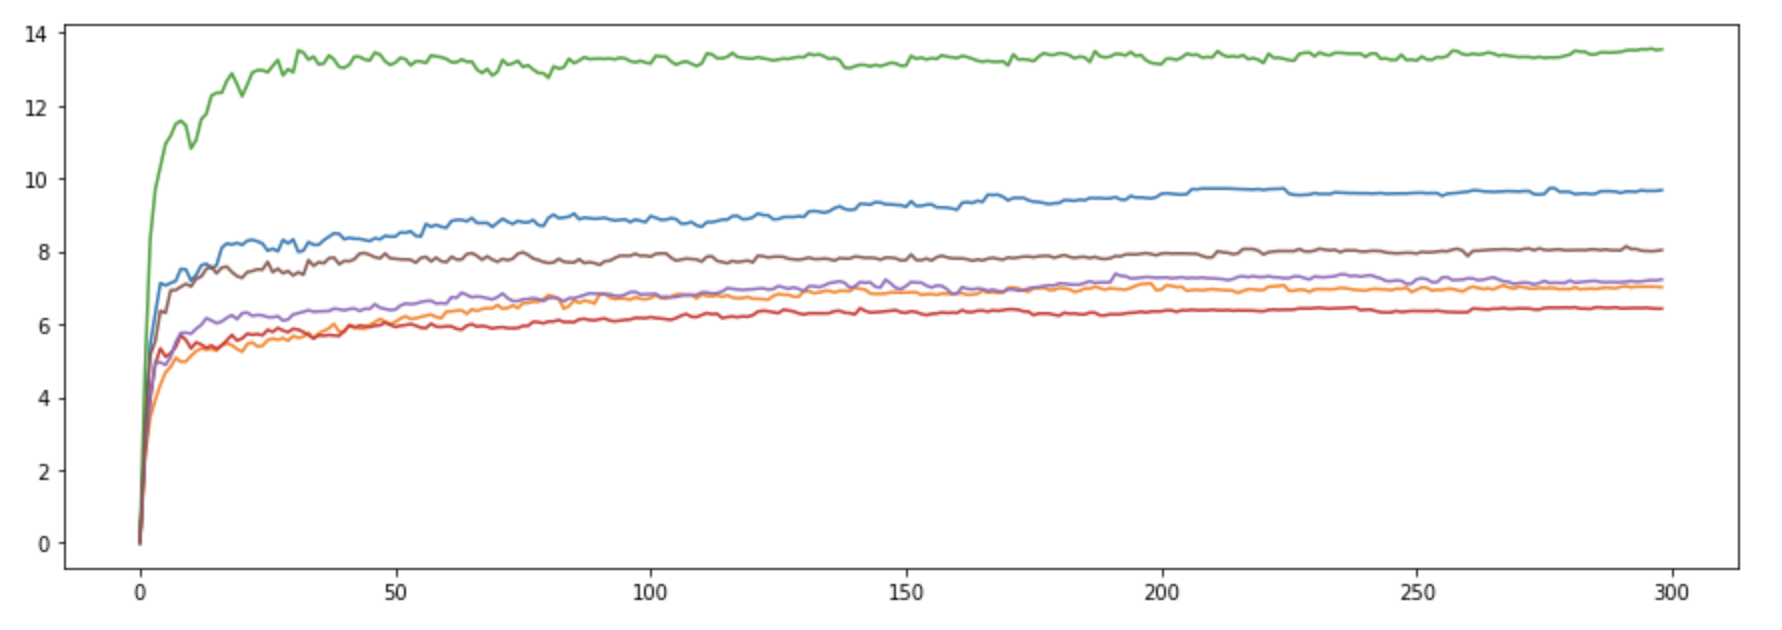
\includegraphics[width=0.4\textwidth]{kneighbor_crps}

\subsection{Gradient Boosted Tree}

We modify the cost function to calculate the . This means that we need to train a model for each of the percentiles we want to
forecast. The other problem is that the percentiles can cross. We will use the method in order to correct that.

\subsection{Quantile Random Forest}

The quantile random forest is based on the usual random forest. The diferent trees create partitions out of the data and 
they select a partition in order to make the prediction. However, this time, the targets on the partition are not aggregated,
but are used to create a distribution function.


\label{sec:mm}

\subsection{Protocol for high \no concentration episodes}
\label{sec:madr-prot-high}


\subsection{Nitrogen dioxide data}
\label{sec:no2}


\subsection{Weather data}
\label{sec:weather-data}

\subsection{ECMWF numerical pollution prediction}
\label{sec:ecmwf-numer-poll}


\subsection{Experimental design}
\label{sec:experimental-design}

\subsection{Evaluation of probabilistic forecasts}
\label{sec:eval-prob-forec}


\subsection{Evaluation of alert forecasting}
\label{sec:eval-extr-value}


\section{Results and discussion}
\label{sec:results}


\subsection{Reference models}
\label{sec:deterministic}

In the first experiment, we used quantile regression to compute
point-forecasts of the expected value (median) for one-day ahead
predictions of \no concentrations.

% latex table generated in R 3.2.2 by xtable 1.7-4 package
% Thu Mar 31 18:48:22 2016
\begin{table}[tbp]
\caption{\label{tab:determ}Point forecast error measures for reference
models (persistence, linear regression, random forests and median of
the probabilistic model (QRF).}
  \centering
\begin{tabular}{rrrrr}
  \toprule
 & RMSE & MAE & Bias & Corr \\ 
  \midrule
  Persistence & 13.47 & 9.23 & 0.04 & 0.88 \\ 
  LR   & 11.51 & 8.16 & -1.62 & 0.91 \\ 
  RF   & 11.27 & 7.89 & -2.14 & 0.92 \\
  Q50  & 11.30 & 7.63 & -0.27 & 0.91 \\ 
   \bottomrule
\end{tabular}
\end{table}

Table \ref{tab:determ} shows the values of the root mean squared error
(RMSE), mean average error (MAE), bias and correlation for the
aforementioned reference models and the median forecast by the
probabilistic model. As we can see, the median-based model Q50 behaves
well in general compared to the other models, being especially good in
terms of MAE and bias. This might be related to the median being more
robust than the mean in the presence of outliers.

However, in this framework, we are, as a matter of fact, interested in
those outliers, as they precisely are the values which trigger the
activation of the air quality protocol.


\subsection{Probabilistic forecasting of extreme values}
\label{sec:probabilistic}


\subsection{Forecasting the probability of alerts}
\label{sec:alertProb2}


\section{Conclusions}
\label{sec:concl}


\section*{References}

\bibliography{refs_nourl}

\end{document} 
%%% Local Variables:
%%% mode: latex
%%% TeX-master: t
%%% End:
